% vim: expandtab softtabstop=2 shiftwidth=2 foldmethod=marker spell

\section{Song Attributes}
Songs are able to be tagged with attributes, and then sorted by those attributes. This is especially useful when streamers form collaborations, and they want to share a single songlist. By adding attributes to all of the newly added songs for the collaboration, you are able to mass edit them. This allows you to more easily make them active or inactive, allowing these songs to be hidden from the users.

In the table below, you can see an example of how the attributes have been implemented in the current backup file. In the header row, the columns \mbox{\lstinline{ATTRIBUTE=NAME\_OF\_TAG}} have been added and a 0 or 1 are used in the following rows to indicate if the song has that attribute. Attributes are not able to be imported, so these columns must be deleted before importing the songs.


\begin{table}[h!]
\pgfplotstabletypeset[col sep=comma,
  string type,
  columns={title,artist,ATTRIBUTE=Love},
  every head row/.style={before row=\hline,after row=\hline},
  every last row/.style={after row=\hline},
  every even row/.style={before row=\rowcolor[gray]{0.9}},
  every first column/.style={column type/.add={|}{}},
  every column/.style={column type/.add={}{|}},
  ]{src/songlist_import/example.csv}
\caption{Song Attribute Example CSV}
\label{song_attribute_example_table}
\end{table}

\clearpage
On The Song Attributes Page, you can see an overview of the current attributes. The values here should only be set together, and be set to \lstinline{Yes}. When set to \lstinline{No}, the attributes disappear in normal user mode from the songlist, and from the set of all attributes displayed at the top of the songlist. Turning specific attributes off is useful for when a streamer doesn't want to play a specific instrument that day, or when not collaborating with the person the tag refers to. Currently there is no easy way to make all songs with an attribute inactive from this page.

\begin{figure}[ht!]
  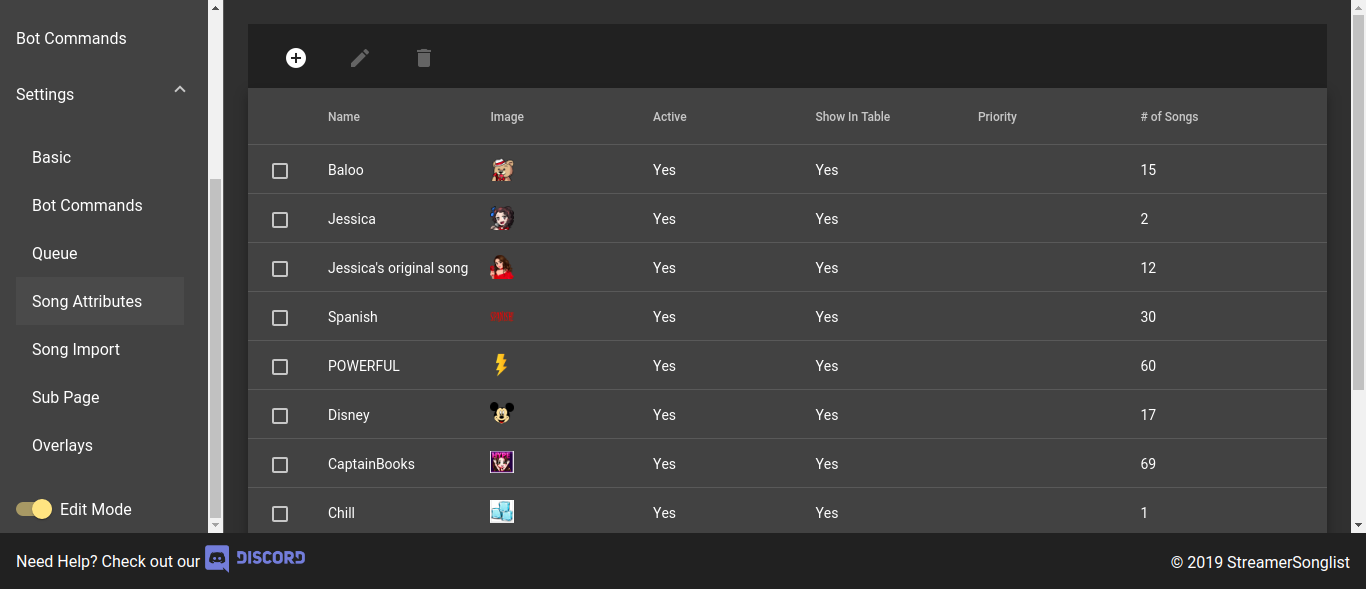
\includegraphics[width=\linewidth]{src/attributes/attributes.png}
  \caption{The Song Attributes page}
  \label{song_attributes_page}
\end{figure}
